\documentclass{article}
\usepackage{amsmath}
\usepackage{amssymb}
\usepackage{chemarr}
\usepackage{hyperref}

\usepackage{graphicx}
\graphicspath{ {./static} }

\setlength{\parindent}{0pt}
\newcommand{\D}{\text{d}}
\let\vec\boldsymbol 

\begin{document}

\title{vbdiff: variational Bayes analysis of simple Brownian mixtures}
\date{February 2024}
\author{Alec Heckert}
\maketitle

\verb|vbdiff| is a simple routine for inference on multi-state Brownian
mixtures. It relies on a variational Bayesian framework to estimate a distribution
over three factors: (1) the diffusion coefficients for each state, (2) the mixing
coefficients, and (3) the origin state for each individual trajectory.
Unlike more sophisticated frameworks like vbSPT, it does not consider state transitions.
As a consequence, it is much faster than these more general models. \newline

Here, we derive \verb|vbdiff|, starting from basic one-state Brownian motion. Many of these results are standard but scattered over different texts; the goal
of this document is provide a unified, accessible introduction to the variational
Brownian mixture model. We also give the evidence lower bound (ELBO) for
\verb|vbdiff| in closed form. This can be used, for example, to choose the
appropriate number of states when modeling a Brownian mixture \cite{bishop2001}.

\tableofcontents

\section{Brownian motion}\label{section:brownian_motion}

A continuous-time stochastic process $B_{t} \in \mathbb{R}$ ($t \in \mathbb{R}$) is Brownian if
\begin{align}
    B_{t} - B_{s} &\sim \mathcal{N} \left( 0, 2 D \left| t - s \right| \right) \qquad &\text{for any $t, s$} \label{eq:rule1} \\
    \text{Cov} \left( B_{t_{1}} - B_{t_{0}}, B_{t_{3}} - B_{t_{2}} \right) &= 0 \qquad &\text{if $t_{0} \leq t_{1} \leq t_{2} \leq t_{3}$} \label{eq:rule2}
\end{align}

where $\mathcal{N} \left( 0, 2 D \left| t - s \right| \right)$ is a normal distribution
with mean 0 and variance $2 D \left| t - s \right|$. \newline

Suppose we measure a Brownian trajectory in a single particle tracking (SPT) experiment.
We sample the particle's position at $m+1$ timepoints
$0, \Delta t, 2 \Delta t, ..., m \Delta t$ where $\Delta t > 0$ is the
frame interval (we'll neglect gaps in the trajectory for now).
Let $\Delta B_{i} = B_{i \Delta t} - B_{(i-1) \Delta t}$ be the
$i^{\text{th}}$ increment (``jump''). Then the joint distribution over
these jumps is
\begin{align*}
    p_{\Delta B_{1}, ..., \Delta B_{m}} \left( \Delta b_{1}, ..., \Delta b_{m} \right) &= \prod\limits_{i=1}^{m} \frac{ \exp \left( - \Delta b_{i}^{2} / 4 D \Delta t \right) }{ \sqrt{ 4 \pi D \Delta t } } \\
    &= \frac{1}{\left( 4 \pi D \Delta t \right)^{m/2}} \exp \left( - \frac{1}{4 D \Delta t} \left[ \Delta b_{1}^{2} + ... + \Delta b_{m}^{2} \right] \right)
\end{align*}

This distribution does not depend on the individual jumps,
only on the sum of their squares. It is straightforward to
show that the sum of squares $X = \Delta B_{1}^{2} + ... + \Delta B_{m}^{2}$
has a gamma distribution. First, the cdf for $\Delta B_{i}^{2}$ is
\begin{align*}
    F_{\Delta B^{2}} \left( x \right) &:= \Pr \left( \Delta B^{2} \leq x \right) \\
    &= \Pr \left( \Delta B \leq \sqrt{x} \right) - \Pr \left( \Delta B < -\sqrt{x} \right) \\
    &= F_{\Delta B} \left( \sqrt{x} \right) - F_{\Delta B} \left( - \sqrt{x} \right)
\end{align*}

Differentiating both sides, we obtain the pdf
\begin{align*}
    f_{\Delta B^{2}}(x) &= \frac{\partial F_{\Delta B^{2}}(x)}{\partial x} \\
    &= \frac{1}{2 \sqrt{x}} \left(
        f_{\Delta B} \left( \sqrt{x} \right) + f_{\Delta B} \left( - \sqrt{x} \right)
    \right)
\end{align*}

Substituting the normal distribution from equation \ref{eq:rule1} as $f_{\Delta B}$,
we have
\[
    f_{\Delta B^{2}}(x) = \frac{ e^{-x / 4 D \Delta t} }{ \sqrt{4 \pi D \Delta t x} }
\]

which we recognize as a gamma distribution with parameters $\alpha = 1/2$ and
$\beta = 1 / 4 D \Delta t$:
\begin{align*}
    \Delta B^{2} &\sim \text{Gamma} \left( \frac{1}{2}, \frac{1}{4 D \Delta t} \right)
\end{align*}

Now, the sum of $m$ independent and identically distributed gamma random variables
with the distribution $\text{Gamma} \left( \alpha, \beta \right)$ has the distribution
$\text{Gamma} \left( m \alpha, \beta \right)$. From this, we have
\begin{equation}
    X := \Delta B_{1}^{2} + ... + \Delta B_{m}^{2} \sim \text{Gamma} \left(
        \frac{m}{2}, \frac{1}{4 D \Delta t}
    \right)
\end{equation}

which corresponds to the pdf
\begin{equation}
    f_{X}(x) = \frac{x^{\frac{m}{2}-1} e^{-x / 4 D \Delta t}}{\Gamma \left( \frac{m}{2} \right) \left( 4 D \Delta t \right)^{m/2}}, \qquad x \geq 0
\end{equation}

Now, suppose that a particle's motion in $d$ spatial dimensions can be
modeled as independent Brownian motions in each dimension. Due to the Pythagorean
theorem, the sum of its squared displacement is now
$X = X_{\text{dimension 1}} + X_{\text{dimension 2}} + ...$, where
the terms on the right-hand side are the sums of its squared displacements along
each spatial dimension. Insofar as these sums are iid, we have
\begin{equation}\label{eq:brownian_likelihood}
    X \sim \text{Gamma} \left( \frac{md}{2}, \frac{1}{4 D \Delta t} \right)
\end{equation}

Frequently, we will find it convenient to parametrize the distribution by
the \emph{scale} parameter $\phi = 4 D \Delta t$ instead of $D$,
in which case the pdf becomes
\begin{equation}\label{eq:brownian_likelihood_2}
    f_{X}(x | \phi) = \frac{x^{\frac{md}{2} - 1} e^{-x / \phi}}{\Gamma \left( \frac{md}{2} \right) \phi^{\frac{md}{2}}}, \quad x \geq 0
\end{equation}

Finally, at the time of writing we are only interested in 2D tracking ($d=2$),
and so the likelihood simplifies to
\begin{align}\begin{split}\label{eq:brownian_likelihood_3}
    X &\sim \text{Gamma} \left( m, \phi \right) \\
    \Rightarrow f_{X}(x | \phi) &= \frac{x^{m-1} e^{-x/\phi}}{\Gamma (m) \phi^{m}}, \quad x \geq 0
\end{split}\end{align}

where as before $\phi = 4 D \Delta t$.
For the sake of readability we use equation \ref{eq:brownian_likelihood_3}
throughout this text, with the understanding that generalizing to $d \neq 2$
requires substituting $m$ with $md / 2$.

\section{Bayesian inference on single-state Brownian motion}

As a building block to mixture models, we first consider a simple
Bayesian model for one-state Brownian motion. Suppose we have a
2D Brownian trajectory with $m$ jumps and sum of squared displacements $x$.
Our goal is to infer a distribution over the scale parameter (diffusion
coefficient) $\phi$ given the observed $x$. Bayes' theorem prescribes
\[
    f_{\phi | X}(\phi | x) \propto f_{X}(x | \phi) f_{\phi}(\phi)
\]

where $f_{X}(x | \phi)$ is given by equation \ref{eq:brownian_likelihood_3}.
For the prior $f_{\phi}(\phi)$, we assume an inverse gamma distribution:
\begin{align*}
    \phi &\sim \text{InvGamma} \left( \alpha_{0}, \beta_{0} \right) \\
    \Rightarrow f_{\phi} \left( \phi \right) &= \frac{\beta_{0}^{\alpha_{0}} e^{-\beta_{0} / \phi}}{\Gamma \left( \alpha_{0} \right) \phi^{\alpha_{0} + 1} }, \quad \phi \geq 0
\end{align*}

Substituting into Bayes' theorem and retaining only factors that depend
directly on $\phi$,
\[
    f_{\phi | X} (\phi | x) \propto \frac{
        e^{-(\beta_{0} + x) / \phi}
    }{
        \phi^{\alpha_{0} + m + 1}
    }
\]

After renormalization, we obtain
\[
    f_{\phi | X} (\phi | x) = \frac{ (\beta_{0} + x)^{\alpha_{0}+m-1} e^{-(\beta_{0} + x) / \phi}}{\Gamma (\alpha_{0} + m) \phi^{\alpha_{0} + m + 1}}
\]

which we recognize as another inverse gamma distribution
\[
    \phi \ | \ X \sim \text{InvGamma} \left( \alpha_{0} + m, \beta_{0} + x \right)
\]

So - due to the conjugacy of the Brownian likelihood \ref{eq:browian_likelihood_3}
and the inverse gamma prior - inference boils down to simply adding
shape and scale parameters. We can obtain a point estimate of the
diffusion coefficient by taking the mean of the posterior distribution:
\[
    \mathbb{E} \left[ D | x \right] = \frac{1}{4 \Delta t} \mathbb{E} \left[ \phi | x \right] = \frac{\beta_{0} + x}{4 \Delta t \left( \alpha_{0} + m - 1 \right)}
\]

Notice that the $-1$ in the denominator is analogous to the Bessel
correction for the sample variance, as the diffusion coefficient is essentially
a variance.

\section{Brownian mixtures}

Most samples of interest in SPT contain a mixture of particles in different
states characterized by distinct diffusion coefficients. Suppose we have a dataset
with $N$ trajectories, each of which originates from one of $K$ distinct states
characterized by scale parameters $\phi_{1}, ..., \phi_{K}$. There are multiple
unknowns here: we don't know the scale parameters for each state, the relative
abundances (``occupations'') of each state, nor which state each trajectory comes
from. To represent this uncertainty, we construct the following mixture model:

\begin{align}\label{eq:brownian_mixture}
    \boldsymbol{\tau} &\sim \text{Dirichlet} \left( \alpha_{0}, ..., \alpha_{0} \right), &\quad \boldsymbol{\tau} \in C^{K-1} \\
    \phi_{j} &\sim \text{InvGamma} \left( \alpha_{0}, \beta_{0} \right), &\quad j \in \left\{ 1, 2, ..., K \right\} \\
    \vec{Z}_{i} \ | \ \boldsymbol{\tau} &\sim \boldsymbol{\tau}, &\quad i \in \left\{ 1, 2, ..., N \right\} \\
    X_{i} \ | \ Z_{ij} = 1, \phi_{j} &\sim \text{Gamma} \left( m_{i}, \phi_{j} \right), &\quad i \in \left\{ 1, 2, ..., N \right\}
\end{align}

Breaking this down:
\begin{itemize}
    \item $\boldsymbol{\tau}$ is an unknown distribution over $K$ states (in other words, it belongs to the simplex $C^{K-1}$).
    \item Each state $j$ is characterized by a scale parameter $\phi_{j}$.
    \item The priors over each $\phi_{j}$ are independent and given by $\text{InvGamma} (\alpha_{0}, \beta_{0})$.
    \item To each observation $i$, we associate a one-hot vector $\vec{Z}_{i} \in \left\{ 0, 1 \right\}^{K}$ so that $Z_{ik} = 1$ if observation $i$ originates from state $j$ and $Z_{ik} = 0$ otherwise. Given knowledge of $\boldsymbol{\tau}$, the event $Z_{ij} = 1$ has probability $\tau_{j}$.
    \item $m_{i}$ is the number of jumps in trajectory $i$.
    \item $X_{i}$ is the sum of squared displacements for trajectory $i$.
\end{itemize}

We will use $\vec{X} = \left( X_{1}, ..., X_{N} \right)$ and
$\vec{Z} = \left( Z_{1}, ..., Z_{N} \right)$ to represent the sequence of
all $X_{i}$ and $\vec{Z}_{i}$.
Likewise, we'll use $\boldsymbol{\phi} = (\phi_{1}, ..., \phi_{K})$ to represent the sequence of scale parameters for all $K$ states.
Then the total probability function for this model factors as
\[
    p \left( \vec{X}, \vec{Z}, \boldsymbol{\tau}, \boldsymbol{\phi} \right) = p \left( \vec{X} | \vec{Z}, \boldsymbol{\phi} \right) p \left( \vec{Z} | \boldsymbol{\tau} \right) p \left( \boldsymbol{\tau} \right) p \left( \boldsymbol{\phi} \right)
\]

For later parts, it's useful to write out each of these terms explicitly:
\begin{equation}\label{eq:eqA}
    p \left( \vec{X} | \vec{Z}, \boldsymbol{\phi} \right) = \prod\limits_{i=1}^{N} \prod\limits_{j=1}^{K} \left[
        \frac{ x_{i}^{m_{i}-1} e^{-x_{i} / \phi_{j}}}{\Gamma (m_{i}) \phi_{j}^{m_{i}}}
    \right]^{Z_{ij}}
\end{equation}

\begin{equation}\label{eq:eqB}
    p \left( \vec{Z} | \boldsymbol{\tau} \right) = \prod\limits_{i=1}^{N} \prod\limits_{j=1}^{K} \tau_{j}^{Z_{ij}}
\end{equation}

\begin{equation}\label{eq:eqC}
    p \left( \boldsymbol{\tau} \right) = \frac{1}{B(\alpha_{0}, ..., \alpha_{0})} \prod\limits_{j=1}^{K} \tau_{j}^{\alpha_{0} - 1}
\end{equation}

\begin{equation}\label{eq:eqD}
    p \left( \boldsymbol{\phi} \right) = \prod\limits_{j=1}^{K} \frac{\beta_{0}^{\alpha_{0}} e^{-\beta_{0} / \phi_{j}}}{\Gamma (\alpha_{0}) \phi_{j}^{\alpha_{0} + 1}}
\end{equation}

(Here, $B(\alpha_{0}, ..., \alpha_{0})$ is the multivariate beta function.) \newline

Of all of these parameters, the only one we actually observe is $\vec{X}$.
Our goal is to infer a posterior distribution over the remaining variables
given an observed set of trajectories.

\section{Approximative inference on Brownian mixtures}

Given an observed set of trajectories $\vec{X} = (X_{1}, ..., X_{N})$, we
want to infer the probability of the unobserved (latent) variables
$\vec{Z}, \boldsymbol{\tau}, \boldsymbol{\phi}$ in the mixture \ref{eq:brownian_mixture}.
In other words, we want to infer the posterior distribution
$p \left( \vec{Z}, \boldsymbol{\tau}, \boldsymbol{\phi} | \vec{X} \right)$.
Solving this problem exactly is intractable. There are two fallbacks:
(a) approximate the distribution with a finite sequence of samples using
MCMC methods or (b) construct a tractable approximation to the posterior.
In \verb|vbdiff|, we take the latter approach. We follow
a classic variational Bayesian approach and paraphrase certain steps;
for more detail see Bishop's book \cite{bishop2006}. \newline

We will approximate the posterior with a tractable distribution $q$:
\[
    q \left( \vec{Z}, \boldsymbol{\tau}, \boldsymbol{\phi} \right) \approx p \left( \vec{Z}, \boldsymbol{\tau}, \boldsymbol{\phi} | \vec{X} \right)
\]

We will use the evidence lower bound (ELBO) as the objective function for $q$:
\begin{equation}\label{eq:elbo}
    \mathcal{L} \left[ q \right] := \mathbb{E}_{\vec{Z}, \boldsymbol{\tau}, \boldsymbol{\phi} \sim q} \left[
        \log \left(
            \frac{ p \left( \vec{X}, \vec{Z}, \boldsymbol{\tau}, \boldsymbol{\phi} \right)}{ q \left( \vec{Z}, \boldsymbol{\tau}, \boldsymbol{\phi} \right) }
        \right)
    \right]
\end{equation}

By factoring $p \left( \vec{X}, \vec{Z}, \boldsymbol{\tau}, \boldsymbol{\phi} \right) = p \left( \vec{Z}, \boldsymbol{\tau}, \boldsymbol{\phi} | \vec{X} \right) p \left( \vec{X} \right)$ in equation \ref{eq:elbo}, it straightforward to show that maximizing $\mathcal{L} [q]$ corresponds to minimizing the Kullback-Leibler divergence between the true and approximative posteriors, and that $\mathcal{L}[q]$ forms a lower bound on the marginal log likelihood $\log p (\vec{X})$:
\begin{align*}
    \underset{q}{\text{argmax}} \: \mathcal{L}[q] &= \underset{q}{\text{argmin}} \: \text{KL} \left( q(\vec{Z}, \boldsymbol{\tau}, \boldsymbol{\phi}) || p (\vec{Z}, \boldsymbol{\tau}, \boldsymbol{\phi} | \vec{X} ) \right) \\
    \mathcal{L}[q] &\leq \log p (\vec{X})
\end{align*}

This last point is crucial, as it will form the basis for model selection considered later on. For now, notice that $p(\vec{X})$ can be seen as the average probability of the observed data over all possible model parameters $\vec{X}, \boldsymbol{\tau}, \boldsymbol{\phi}$ with some $K$. \newline

What form will we choose for $q$? As it turns out, we only need to make a
single constraint to find a tractable $q$: assume that $q$ factors into
separate distributions over $\vec{Z}$ and $\boldsymbol{\tau}, \boldsymbol{\phi}$:
\[
    q \left( \vec{Z}, \boldsymbol{\tau}, \boldsymbol{\phi} \right) = q \left( \vec{Z} \right) q \left( \boldsymbol{\tau}, \boldsymbol{\phi} \right)
\]

This factorability criterion - a kind of mean field approximation - is sufficient
to completely specify the form of the optimal $q$. It can be shown \cite{bishop2006}
that $\underset{q}{\text{argmax}} \: \mathcal{L}[q]$ satisfies
\begin{align}\begin{split}\label{eq:em_equations}
    \log q \left( \vec{Z} \right) &= \mathbb{E}_{\boldsymbol{\tau}, \boldsymbol{\phi} \sim q (\boldsymbol{\tau}, \boldsymbol{\phi})} \left[ \log p \left( \vec{X}, \vec{Z}, \boldsymbol{\tau}, \boldsymbol{\phi} \right) \right] \\
    \log q \left( \boldsymbol{\tau}, \boldsymbol{\phi} \right) &= \mathbb{E}_{\vec{Z} \sim q(\vec{Z})} \left[ \log p \left( \vec{X}, \vec{Z}, \boldsymbol{\tau}, \boldsymbol{\phi} \right) \right]
\end{split}\end{align}

We solve these equations in Appendix \ref{appendix:derivation_approx_posterior}.
Skipping to the punchline, the optimal approximation $q$ is given by
\begin{align}\begin{split}
    q \left( \vec{Z}, \boldsymbol{\tau}, \boldsymbol{\phi} \right) &= q \left( \vec{Z} \right) q \left( \boldsymbol{\tau} \right) q \left( \boldsymbol{\phi} \right) \\
    q \left( \vec{Z} \right) &= \prod\limits_{i=1}^{N} \prod\limits_{j=1}^{K} r_{ij}^{Z_{ij}} \\
    q \left( \boldsymbol{\tau} \right) &= \text{Dirichlet} \left(
        \boldsymbol{\tau} | \alpha_{0} + \alpha_{1}, ..., \alpha_{0} + \alpha_{K}
    \right) \\
    q \left( \boldsymbol{\phi} \right) &= \prod\limits_{j=1}^{K} \text{InvGamma} \left(
        \phi_{j} | \alpha_{0} + \alpha_{j}, \beta_{0} + \beta_{j}
    \right)
\end{split}\end{align}

where
\begin{align}\begin{split}
    r_{ij} &= \frac{
        \exp \left(
            \mathbb{E}_{q} \left[ \log \tau_{j} \right] - x_{i} \mathbb{E}_{q} \left[ \phi_{j}^{-1} \right] - m_{i} \mathbb{E}_{q} \left[ \log \phi_{j} \right]
        \right)
    }{
        \sum\limits_{k=1}^{K} \exp \left(
            \mathbb{E}_{q} \left[ \log \tau_{k} \right] - x_{i} \mathbb{E}_{q} \left[ \phi_{k}^{-1} \right] - m_{i} \mathbb{E}_{q} \left[ \log \phi_{k} \right]
        \right)
    } \\
    \alpha_{j} &= \sum\limits_{i=1}^{N} \mathbb{E}_{q} \left[ Z_{ij} \right] m_{i} \\
    \beta_{j} &= \sum\limits_{i=1}^{N} \mathbb{E}_{q} \left[ Z_{ij} \right] x_{i}
\end{split}\end{align}

Inference consists of cyclically updating $r_{ij}$, $\alpha_{j}$, and $\beta_{j}$
until convergence. This can be done by substituting the following expectations at each update:
\begin{align*}
    \mathbb{E}_{q} \left[ Z_{ij} \right] &= r_{ij} \\
    \mathbb{E}_{q} \left[ \log \tau_{j} \right] &= \psi \left( \alpha_{0} + \alpha_{j}) - \psi (K \alpha_{0} + \alpha_{1} + ... + \alpha_{K} \right) \\
    \mathbb{E}_{q} \left[ \phi_{j}^{-1} \right] &= \frac{\alpha_{0} + \alpha_{j}}{\beta_{0} + \beta_{j}} \\
    \mathbb{E}_{q} \left[ \log \phi_{j} \right] &= \log (\beta_{0} + \beta_{j}) - \psi (\alpha_{0} + \alpha_{j})
\end{align*}

\subsection{Choice of hyperparameters}

There are three hyperparameters in the mixture model \ref{eq:brownian_mixture}:
\begin{itemize}
    \item $\alpha_{0}$, the pseudocounts accorded to each state in the prior;
    \item $\beta_{0}$, the prior scale parameter for each state;
    \item $K$, the number of states.
\end{itemize}

The last ($K$) is treated in the next section \ref{section:elbo}. The number of pseudocounts is often set to $\alpha_{0} = 2$ in \verb|vbdiff|, to avoid division by zero when evaluating prior means. For $\beta_{0}$, suppose we have some prior guess for the diffusion coefficient $D_{0}$. Since $\phi = 4 D \Delta t$ and the prior mean value of $\phi$ is $\beta_{0} / (\alpha_{0} - 1)$, a sensible choice is to set $\beta_{0} = 4 \Delta t (\alpha_{0} - 1) D_{0}$. This corresponds to the average sum of squared displacements for a trajectory with $\alpha_{0}$ jumps and diffusion coefficient $D_{0}$, sampled with frame interval $\Delta t$.

\section{Evidence lower bound (ELBO)}\label{section:elbo}

A central hyperparameter in the mixture model \ref{eq:brownian_mixture} is the number of states $K$. How do we choose $K$ in a principled way? \newline

Besides providing an objective function for variational Bayesian inference,
the evidence lower bound \ref{eq:elbo} can also be used for \emph{model selection}. Because $\mathcal{L}[q] \leq \log p \left( \vec{X} \right)$, the ELBO provides an approximation to the probability of the observed data $\vec{X}$ averaged over all model parameters $\vec{X}, \boldsymbol{\tau}, \boldsymbol{\phi}$ corresponding to a particular $K$. If $K$ is too small, then there may not exist model parameters that adequately describe the data. If $K$ is too high, then even if model parameters exist that adequately describe the data, most do not. In short, we should take the $K$ with the highest $\mathcal{L}[q]$. \newline

Expanding the ELBO equation \ref{eq:elbo}, we have
\begin{align}
    \mathcal{L} [q] &= \mathbb{E}_{q} \left[ \log p \left( \vec{X} | \vec{Z}, \boldsymbol{\tau}, \boldsymbol{\phi} \right) \right] \quad &\text{(term A)} \\
    &\quad + \mathbb{E}_{q} \left[ \log p \left( \vec{Z} | \boldsymbol{\tau} \right) \right] \quad &\text{(term B)} \\
    &\quad + \mathbb{E}_{q} \left[ \log p \left( \boldsymbol{\tau} \right) \right] \quad &\text{(term C)} \\
    &\quad + \mathbb{E}_{q} \left[ \log p \left( \boldsymbol{\phi} \right) \right] \quad &\text{(term D)} \\
    &\quad - \mathbb{E}_{q} \left[ \log q \left( \vec{Z} \right) \right] \quad &\text{(term E)} \\
    &\quad - \mathbb{E}_{q} \left[ \log q \left( \boldsymbol{\tau} \right) \right] \quad &\text{(term F)} \\
    &\quad - \mathbb{E}_{q} \left[ \log q \left( \boldsymbol{\phi} \right) \right] \quad &\text{(term G)}
\end{align}

Separately, these terms are:
\begin{align*}
    \mathbb{E}_{q} \left[ \log p \left( \vec{X} | \vec{Z}, \boldsymbol{\tau}, \boldsymbol{\phi} \right) \right] &= \sum\limits_{i=1}^{N} \sum\limits_{j=1}^{K} \mathbb{E}_{q} \left[ Z_{ij} \right] \Big(
        (m_{i} - 1) \log x_{i} - \log \Gamma (m_{i}) \\
    &\qquad - m_{i} \mathbb{E}_{q} \left[ \log \phi_{j} \right] - x_{i} \mathbb{E}_{q} \left[ \phi_{j}^{-1} \right] \Big) \\
    \mathbb{E}_{q} \left[ \log p \left( \vec{Z} | \boldsymbol{\tau} \right) \right] &= \sum\limits_{i=1}^{N} \sum\limits_{j=1}^{K} \mathbb{E}_{q} \left[ Z_{ij} \right] \mathbb{E}_{z} \left[ \log \tau_{j} \right] \\
    \mathbb{E}_{q} \left[ \log p \left( \boldsymbol{\tau} \right) \right] &= - \log B (\alpha_{0}, ..., \alpha_{0}) + \sum\limits_{j=1}^{K} (\alpha_{0} - 1) \mathbb{E}_{q} \left[ \log \tau_{j} \right] \\
    \mathbb{E}_{q} \left[ \log p \left( \boldsymbol{\phi} \right) \right] &= \sum\limits_{j=1}^{K} \left(
        \alpha_{0} \log \beta_{0} - \log \Gamma (\alpha_{0}) - \beta_{0} \phi_{j}^{-1} - (\alpha_{0} + 1) \log \phi_{j}
    \right) \\
    \mathbb{E}_{q} \left[ \log q \left( \vec{Z} \right) \right] &= \sum\limits_{i=1}^{N} \sum\limits_{j=1}^{K} \mathbb{E}_{q} \left[ Z_{ij} \right] \log r_{ij} \\
    \mathbb{E}_{q} \left[ \log q \left( \boldsymbol{\tau} \right) \right] &= - \log B (\alpha_{0} + \alpha_{1}, ..., \alpha_{0} + \alpha_{K} ) + \sum\limits_{j=1}^{K} (\alpha_{0} + \alpha_{j} - 1) \mathbb{E}_{q} \left[ \log \tau_{j} \right] \\
    \mathbb{E}_{q} \left[ \log q \left( \boldsymbol{\phi} \right) \right] &= \sum\limits_{j=1}^{K} \Big(
        (\alpha_{0} + \alpha_{j}) \log (\beta_{0} + \beta_{j}) - \log \Gamma (\alpha_{0} + \alpha_{j}) \\
    &\qquad - (\beta_{0} + \beta_{j}) \mathbb{E}_{q} \left[ \phi_{j}^{-1} \right] - (\alpha_{0} + \alpha_{j} + 1) \mathbb{E}_{q} \left[ \log \phi_{j} \right] 
    \Big)
\end{align*}

where, as before, $B(x_{1}, ..., x_{K})$ is the multivariate beta function and the inner expectations are given by
\begin{align*}
    \mathbb{E}_{q} \left[ Z_{ij} \right] &= r_{ij} \\
    \mathbb{E}_{q} \left[ \phi_{j}^{-1} \right] &= \frac{\alpha_{0} + \alpha_{j}}{\beta_{0} + \beta_{j}} \\
    \mathbb{E}_{q} \left[ \log \phi_{j} \right] &= \log (\beta_{0} + \beta_{j}) - \psi (\alpha_{0} + \alpha_{j}) \\
    \mathbb{E}_{q} \left[ \log \tau_{j} \right] &= \psi (\alpha_{0} + \alpha_{j}) - \psi (K \alpha_{0} + \alpha_{1} + ... + \alpha_{k} )
\end{align*}

where $\psi$ is the digamma function.

\begin{figure}
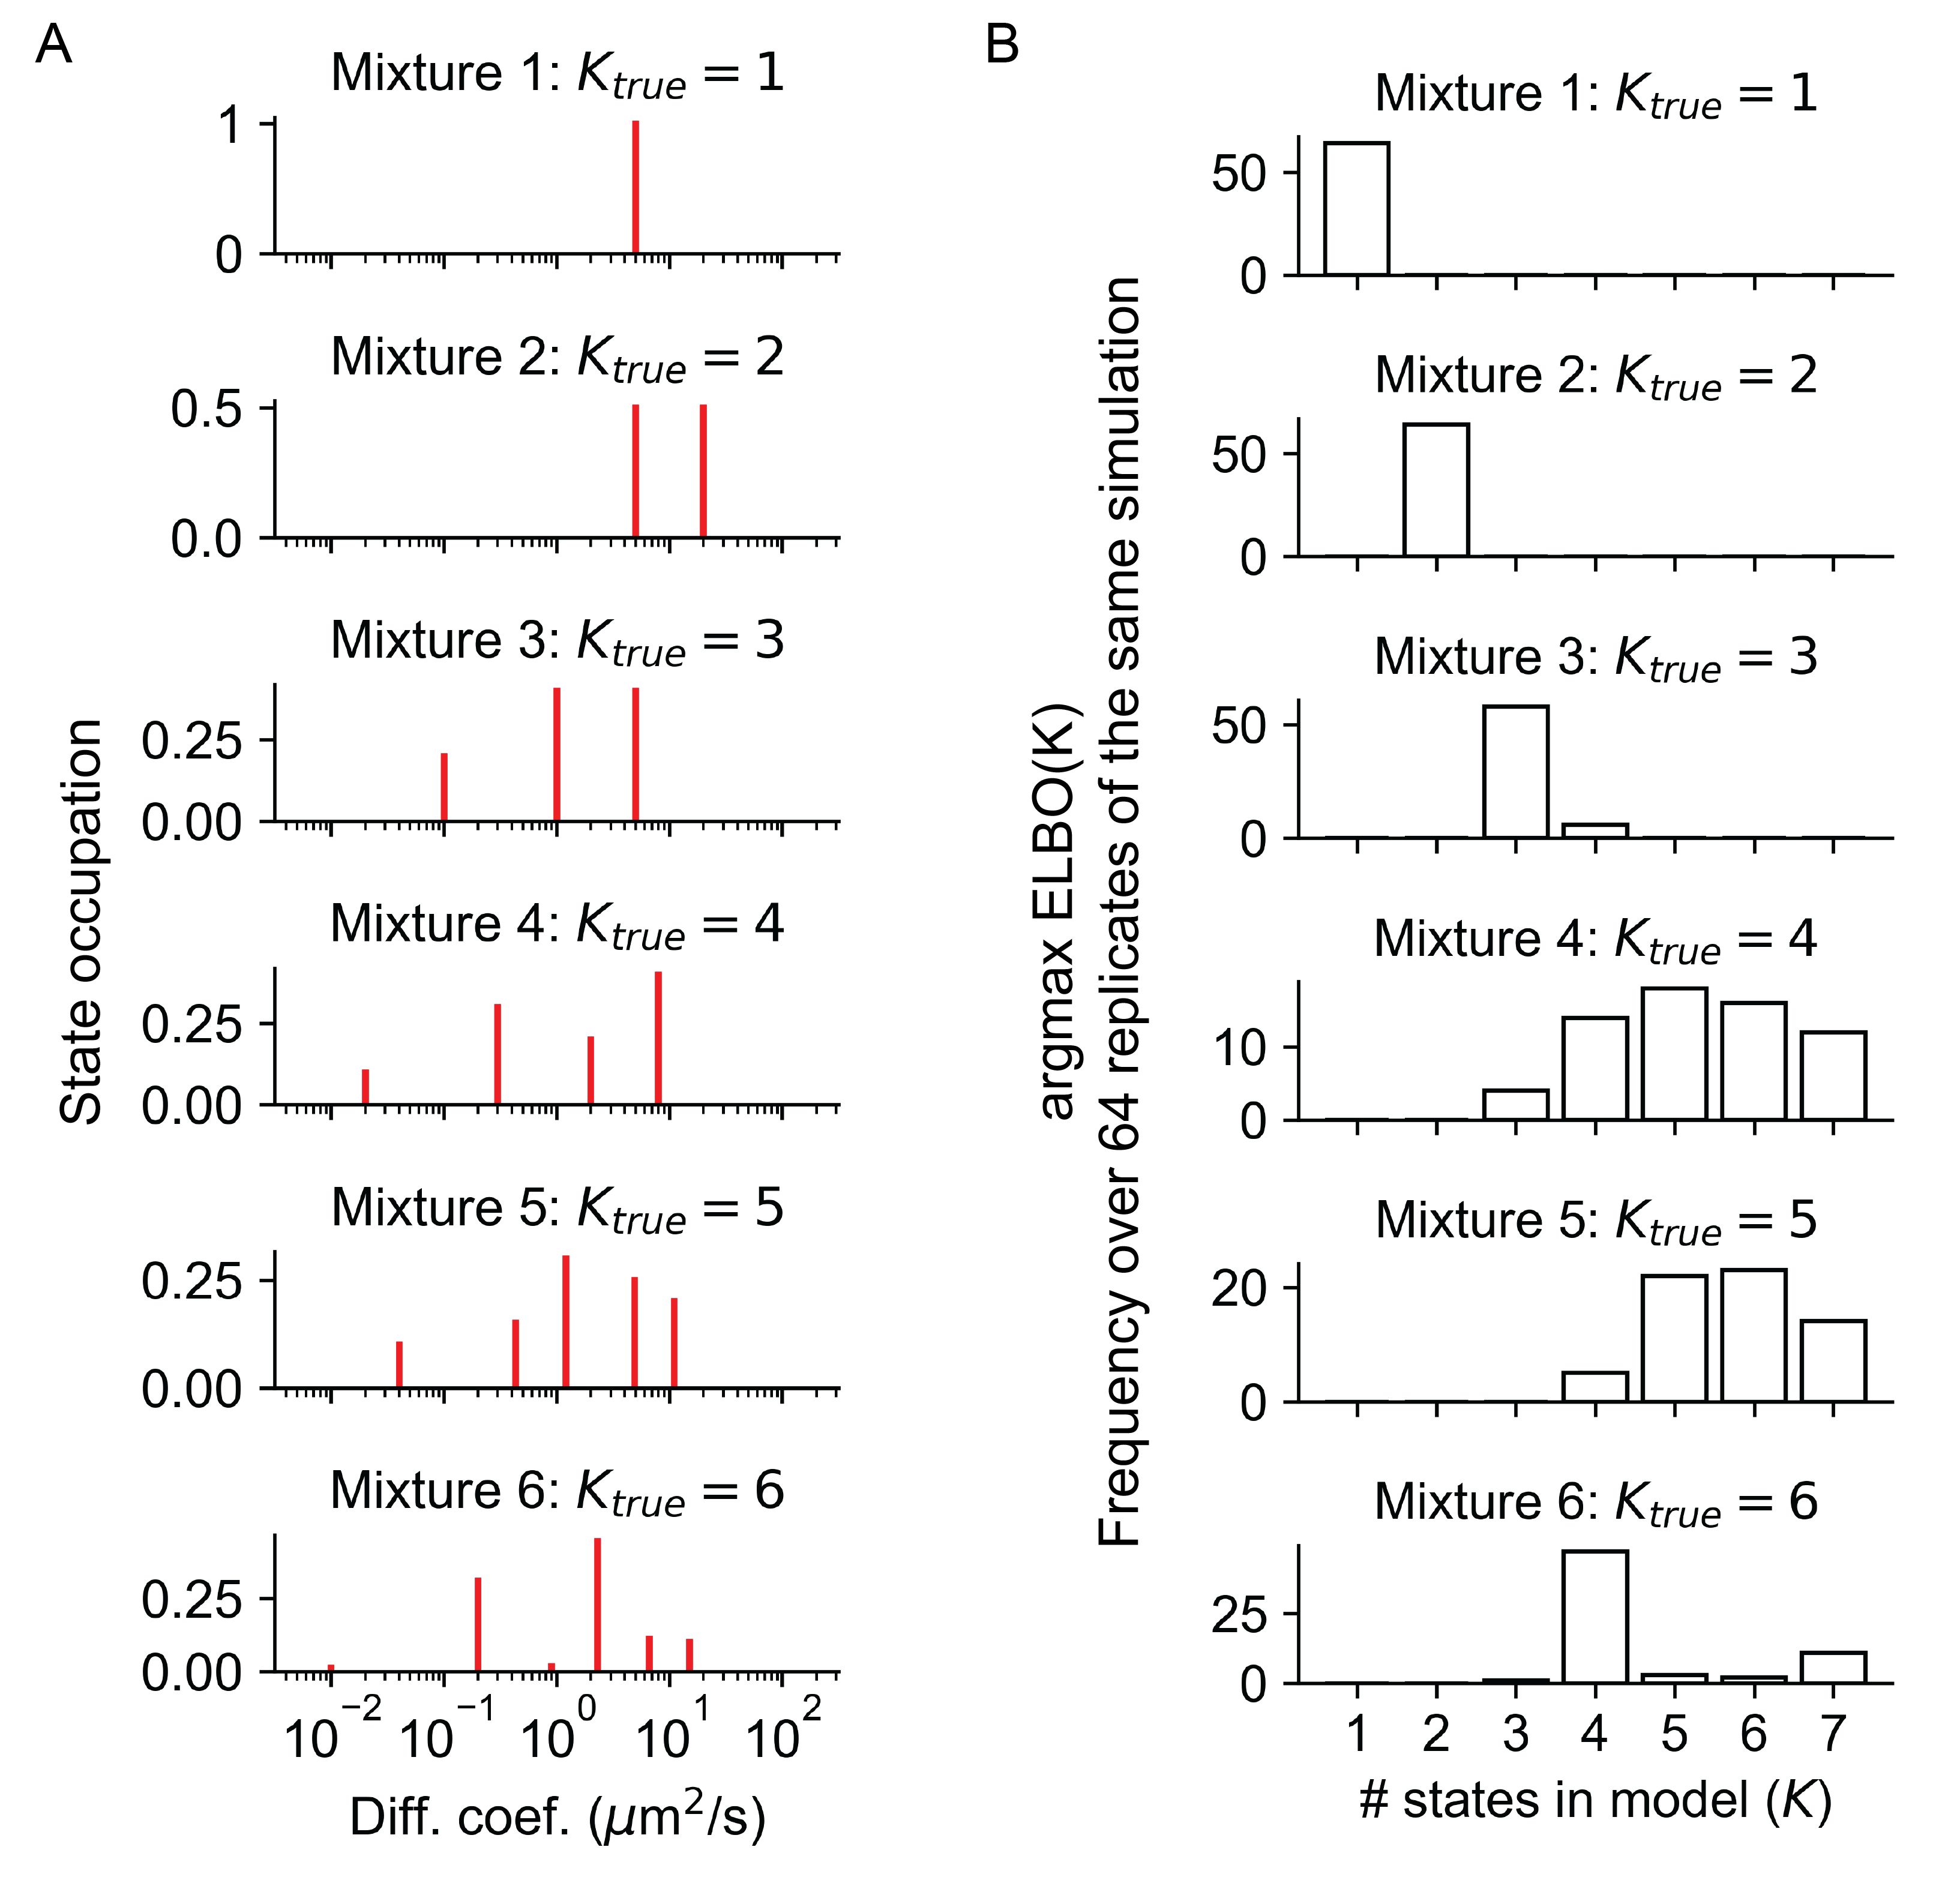
\includegraphics[width=0.55\pagewidth]{elbo_comparison.png}
\caption{Using the ELBO to determine the number of states $K$ in a Brownian mixture. We simulated Brownian mixtures with different numbers of states ($K_{\text{true}}$), then attempted to recover the correct $K$ using vbdiff. To do this, we fit each simulated mixture to models with $K=1$, 2, 3, 4, 5, 6, or 7 and took the $K$ with the highest ELBO. Brownian mixture simulations were performed with the \href{https://github.com/alecheckert/strobesim}{strobesim} package, which simulates SPT-like conditions including 20 nm localization error, 700 nm depth of field, bleaching rate 10 Hz, frame rate 200 Hz, and approximately 7000 observed trajectories per simulation. Mean trajectory length is $\sim 3-4$ frames under these conditions (depending on the simulation). (A) Each of the six Brownian mixtures simulated. Red bars indicate ground truth states and the height of the bars indicates each state's \emph{occupation} - the fraction of particles originating from that state. (B) Histogram of recovered $K$ over 64 replicates of each simulated mixture. Notice that uncertainty in $K$ rises as $K_{\text{true}}$ rises.}
\end{figure}

\section{Addressing experimental biases}

\verb|vbdiff| also incorporates two experimental biases common
in SPT experiments: localization error and defocalization.

\subsection{Localization error}

In real SPT experiments, the position of a particle isn't known exactly,
but is always associated with some measurement error (known as
\emph{localization error}). We model a Brownian motion with
localization error as the process $\tilde{B}_{t} = B_{t} + \sigma_{\text{loc}} W_{t}$
where $B_{t}$ is a Brownian motion, $W_{t}$ is a Gaussian white noise process,
and $\sigma_{\text{loc}}^{2}$ is the localization error variance. \newline

If the particle's position is measured at regular timepoints $0, \Delta t, 2 \Delta t, ...$
so that the $i^{\text{th}}$ increment is $\Delta \tilde{B}_{i} = \tilde{B}_{i \Delta t} - \tilde{B}_{(i-1) \Delta t}$, then the increments have the covariance
\[
    \text{Cov} \left( \Delta \tilde{B}_{i}, \Delta \tilde{B}_{j} \right) = \begin{cases}
        2 D \Delta t + 2 \sigma_{\text{loc}}^{2} \qquad &\text{if } i = j \\
        - \sigma_{\text{loc}}^{2} \qquad &\text{if } \left| i - j \right| = 1 \\
        0 \qquad &\text{otherwise}
    \end{cases}
\]

Models that incorporate the full covariance function, including the negative
covariance between sequential jumps, include \href{https://github.com/alecheckert/saspt}{state arrays}. State arrays also allow each trajectory to have a distinct
localization error. In \verb|vbdiff| we take a simpler approach by neglecting the
off-diagonal covariances and assuming that localization error variance is a known
constant, identical for all trajectories. Then the same arguments
from Section \ref{section:brownian_motion} generate the likelihood function
\begin{equation}
    X_{i} | D_{j}, \sigma_{\text{loc}}^{2} \sim \text{Gamma} \left( \frac{m_{i} d}{2}, \frac{1}{4 (D_{j} \Delta t + \sigma_{\text{loc}}^{2} )} \right)
\end{equation}

where $X$ is the sum of squared displacements in trajectory $i$,
$D_{j}$ is the diffusion coefficient for the $j^{\text{th}}$ state,
$m_{i}$ is the number of trajectories in trajectory $i$, and $d$
is the spatial dimension (usually 2). The core \verb|vbdiff| algorithm
remains exactly the same, except we define
$\phi_{j} = 4 (D \Delta t + \sigma_{\text{loc}}^{2})$ as the parameter
for each state.

\subsection{Defocalization}

In real SPT experiments, particles are only observed when their
positions coincide with the imaging system's depth of field.
As a result, the jumps of fast particles are more likely to land outside
the depth of field than the jumps of slow particles, creating a state
bias toward slow particles. \newline

In \verb|vbdiff|, we address this bias in the following way.
Suppose, as before, that the ``observed'' state occupations
are represented by $\boldsymbol{\tau} = (\tau_{1}, \tau_{2}, ..., \tau_{K})$.
Let $\eta_{j}(\phi_{j})$ be the probability to observe a jump from state $j$ given its mobility parameter $\phi_{j}$ and the imaging system's depth of field.
Then the ``true'' state occupations are some vector
$\boldsymbol{\mu} = (\mu_{1}, \mu_{2}, ..., \mu_{K})$ such that
$\sum_{j=1}^{K} \mu_{j} = 1$ and
\begin{equation}\label{eq:observed_occ}
    \tau_{j} = \frac{ \eta_{j} (\phi_{j}) \mu_{j} }{ \sum\limits_{k=1}^{K} \eta_{k} (\phi_{k}) \mu_{k} }
\end{equation}

(Note: We could also incorporate photobleaching into $\eta_{j} (\phi_{j})$. But
since we usually assume photobleaching affects all states equally,
it factors out from the numerator and denominator in equation
\ref{eq:observed_occ} and we're left with only the defocalization part.) \newline

We can include this in the stochastic model by modifying
equation \ref{eq:eqB} so that it incorporates both the
probability to sample a particle in state $j$ ($\mu_{j}$)
as well as the probability to observe a jump from that
particle ($\eta_{j}(\phi_{j})$):
\[
    \log p \left( \vec{Z} | \boldsymbol{\mu}, \boldsymbol{\phi} \right) \propto \sum\limits_{i=1}^{N} \sum\limits_{j=1}^{K} Z_{ij} \left(
        \log \eta_{j} (\phi_{j}) + \log \mu_{j}
    \right)
\]

To make things simpler, we will assume that $\eta_{j}$ is constant
at each iteration of \verb|vbdiff|. For instance, we can 
evaluate $\eta_{j}$ at the current posterior mean value of $\phi_{j}$.
Then
\[
    \log p \left( \vec{Z} | \boldsymbol{\mu} \right) \propto \sum\limits_{i=1}^{N} \sum\limits_{j=1}^{K} Z_{ij} \left(
        \log \eta_{j} + \log \mu_{j}
    \right)
\]

To understand how to incorporate this into the \verb|vbdiff|
algorithm, it is useful to examine the max likelihood solution to
$\hat{\boldsymbol{\mu}} = \underset{\boldsymbol{\mu}}{\text{argmax}} \: p \left( \vec{Z} | \boldsymbol{\mu} \right)$. 
We seek the $\boldsymbol{\mu}$ that maximizes the Lagrangian
\[
    L(\boldsymbol{\mu}, \lambda) = \sum\limits_{i=1}^{N} \sum\limits_{j=1}^{K} Z_{ij} \left(
        \log \eta_{j} + \log \mu_{j}
    \right) - \lambda \sum\limits_{j=1}^{K} \eta_{j} \mu_{j}
\]

where $\lambda$ is a Lagrange multiplier corresponding to the
normalization constraint $\sum_{j=1}^{K} \eta_{j} \mu_{j} = 1$.
Taking the first derivative with respect to $\mu_{j}$ and $\lambda$,
setting to zero, and solving the resulting system of equations gives
\[
    \hat{\mu}_{j} = \frac{\eta_{j}^{-1} \tau_{j}}{\sum\limits_{k=1}^{K} \eta_{k}^{-1} \tau_{k}}
\]

where we have used $\tau_{j} = \frac{1}{N} \sum\limits_{i=1}^{N} Z_{ij}$
to paraphrase the result. This simple correction suggests that
in the update scheme for \verb|vbdiff| we should adjust the
occupations for state $j$ by a factor proportional to $\eta_{j}^{-1}$:
\[
    q \left( \boldsymbol{\tau} \right) = \text{Dirichlet} \left(
        \alpha_{0} + \overline{\eta}_{1}^{-1} \alpha_{1},
        ...,
        \alpha_{0} + \overline{\eta}_{K}^{-1} \alpha_{K}
    \right)
\]

where $\overline{\eta}_{j} \propto \eta_{j}$ such that the overall
statistical weight of the trajectories (number of jumps in the dataset)
is unchanged. \newline

In \verb|vbdiff|, we evaluate $\eta_{j} = \eta_{j} (\phi_{j})$
at each iteration using a numerical propagator approach
(see \verb|emdiff/defoc.py|).

\appendix

\section{Appendix A: Derivation of approximate posterior for Brownian mixtures}\label{appendix:derivation_approx_posterior}

To identify the exact form of the approximative posterior $q(\vec{X}, \boldsymbol{\tau}, \boldsymbol{\phi})$ for Brownian mixtures, we will solve the system of equations \ref{eq:em_equations} given the model specified by \ref{eq:eqA}, \ref{eq:eqB}, \ref{eq:eqC}, and \ref{eq:eqD}. \newline

First we consider the second equation in \ref{eq:em_equations}. Writing this out,
\begin{align}\begin{split}\label{eq:int1}
    \log q \left( \boldsymbol{\tau}, \boldsymbol{\phi} \right) &= \mathbb{E}_{\vec{Z} \sim q(\vec{Z})} \left[ \log p \left( \vec{X}, \vec{Z}, \boldsymbol{\tau}, \boldsymbol{\phi} \right) \right] \\
    &= \sum\limits_{j=1}^{K} \left( \alpha_{0} - 1 + \sum\limits_{i=1}^{N} \mathbb{E}_{q} \left[ Z_{ij} \right] m_{i} \right) \log \tau_{j} \\
    &\quad - \sum\limits_{j=1}^{K} \left( \beta_{0} + \sum\limits_{i=1}^{N} \mathbb{E}_{q} \left[ Z_{ij} \right] x_{i} \right) \phi_{j}^{-1} \\
    &\quad - \sum\limits_{j=1}^{K} \left(
        \alpha_{0} + 1 + \sum\limits_{i=1}^{N} \mathbb{E}_{q} \left[ Z_{ij} \right] m_{i}
    \right) \log \phi_{j} \\
    &\qquad + \text{constant}
\end{split}\end{align}

where the constant collects all terms that do not directly depend
on $\boldsymbol{\tau}$ or $\boldsymbol{\phi}$. We have made one
arbitrary modification in equation \ref{eq:int1}, weighting the statistical
weight of trajectory $i$ toward state $j$ by its number of jumps $m_{i}$
rather than the same for all tracks. This accounts for a bias unmodeled
by the naive mixture \ref{eq:brownian_mixture} - fast states tend to produce
many short trajectories while slow states tend to produce a few long trajectories. Weighting statistical weight by the number of jumps in each trajectory removes some of this bias; the remaining bias can be addressed via defocalization corrections. \newline

Examining the form of equation \ref{eq:int1}, we see that it is a product
of a Dirichlet distribution over $\boldsymbol{\tau}$ and independent inverse
gamma distributions over each scale parameter $\phi_{j}$:
\begin{align}\begin{split}\label{eq:int2}
    q \left( \boldsymbol{\tau}, \boldsymbol{\phi} \right) &= q \left( \boldsymbol{\tau} \right) \prod\limits_{j=1}^{K} q \left( \phi_{j} \right) \\
    q \left( \boldsymbol{\tau} \right) &= \text{Dirichlet} \left( \boldsymbol{\tau} \ | \ \alpha_{0} + \alpha_{1}, ..., \alpha_{0} + \alpha_{K} \right) \\
    q \left( \phi_{j} \right) &= \text{InvGamma} \left(
        \alpha_{0} + \alpha_{j}, \beta_{0} + \beta_{j}
    \right) \\
    \alpha_{j} &= \sum\limits_{i=1}^{N} \mathbb{E}_{q} \left[ Z_{ij} \right] m_{i} \\
    \beta_{j} &= \sum\limits_{i=1}^{N} \mathbb{E}_{q} \left[ Z_{ij} \right] x_{i}
\end{split}\end{align}

We still need to solve $q(\vec{Z})$. Expanding the first equation
in \ref{eq:em_equations}, we have
\begin{align*}
    \log q \left( \vec{Z} \right) &= \mathbb{E}_{\boldsymbol{\tau}, \boldsymbol{\phi} \sim q (\boldsymbol{\tau}, \boldsymbol{\phi})} \left[ \log p \left( \vec{X}, \vec{Z}, \boldsymbol{\tau}, \boldsymbol{\phi} \right) \right] \\
    &= \sum\limits_{i=1}^{N} \sum\limits_{j=1}^{K} Z_{ij} \Big(
        \mathbb{E}_{q} \left[ \log \tau_{j} \right] + (m_{i}-1) \log x_{i} - x_{i} \mathbb{E}_{q} \left[ \phi_{j}^{-1} \right] \\
    &\quad - \log \Gamma (m_{i}) - m_{i} \mathbb{E}_{q} \left[ \log \phi_{j} \right] \Big) + \text{constant}
\end{align*}

where, as before, we've aggregated terms that do not depend on $\vec{Z}$
into the constant.
Normalizing over all states for each trajectory $i$, we have
\begin{align}\begin{split}\label{eq:int3}
    q \left( \vec{Z} \right) &= \prod\limits_{i=1}^{N} \prod\limits_{j=1}^{K} r_{ij}^{Z_{ij}} \\
    r_{ij} &= \frac{
        \exp \left(
            \mathbb{E}_{q} \left[ \log \tau_{j} \right] - x_{i} \mathbb{E}_{q} \left[ \phi_{j}^{-1} \right] - m_{i} \mathbb{E}_{q} \left[ \log \phi_{j} \right]
        \right)
    }{
        \sum\limits_{k=1}^{K} \exp \left(
            \mathbb{E}_{q} \left[ \log \tau_{k} \right] - x_{i} \mathbb{E}_{q} \left[ \phi_{k}^{-1} \right] - m_{i} \mathbb{E}_{q} \left[ \log \phi_{k} \right]
        \right)
    }
\end{split}\end{align}

Together, equations \ref{eq:int2} and \ref{eq:int3} specify the approximative posterior. The expectation-maximization routine cyclically updates the expectations in these equations, obtaining a progressively better estimate of the posterior. Convergence is guaranteed because the ELBO is convex with respect to each factor in $q$ \cite{boyd2004}. Since we know the forms of $q(\vec{Z})$, $q(\boldsymbol{\tau})$, and $q(\boldsymbol{\phi})$, the updates for each expectation can be evaluated in closed form:
\begin{align*}
    \mathbb{E}_{q} \left[ Z_{ij} \right] &= r_{ij} \\
    \mathbb{E}_{q} \left[ \tau_{j} \right] &= \psi \left( \alpha_{0} + \alpha_{j} \right) - \psi \left( K \alpha_{0} + \alpha_{1} + ... + \alpha_{K} \right) \\
    \mathbb{E}_{q} \left[ \phi_{j}^{-1} \right] &= \frac{\alpha_{0} + \alpha_{j}}{\beta_{0} + \beta_{j}} \\
    \mathbb{E}_{q} \left[ \log \phi_{j} \right] &= \log (\beta_{0} + \beta_{j}) - \psi ( \alpha_{0} + \alpha_{j} )
\end{align*}

where $\alpha_{j}, \beta_{j}$ are defined as in equation \ref{eq:int2} and
$\psi(\tau) = \frac{\partial}{\partial \tau} \log \Gamma (\tau)$ is the
digamma function.

\begin{thebibliography}{9}

\bibitem{bishop2001}
Corduneanu A. \& Bishop C. M. Variational Bayesian model selection for mixture distributions. \emph{Artificial Intelligence and Statistics}, 27-34 (2001).

\bibitem{bishop2006}
Bishop C. M. \emph{Pattern Recognition and Machine Learning}. Springer (2006).

\bibitem{boyd2004} 
Boyd S. \& Vandenberghe L. \emph{Convex Optimization}. Cambridge University Press (2004).

\end{thebibliography}

\end{document}
